
\chapter{智能，成于计算机 \texorpdfstring{\\}{ }简明AI史}

 \begin{introduction}
  \item Definition of Theorem
  \item Ask for help
  \item Optimization Problem
  \item Property of Cauchy Series
  \item Angle of Corner
\end{introduction}

\cnquote{}{ 傅鹰}
\cnquote{}{约翰·冯·诺伊曼}
                

人工智能（AI）的发展史和数学史一样，是一部不断突破技术限制、追求理解智能本质的进化历程。从最初的理论奠基，到今天无处不在的智能应用，AI的发展经历了多个阶段，每一个阶段都为未来奠定了新的基础。

\section{AI的萌芽期：理论的起源与计算机的诞生}
AI的概念可以追溯到20世纪中叶，然而其理论根基则来自更早的数学与逻辑学研究。
事实上，AI的出现并非偶然，它是人类在探索计算的更高效率和智能模拟道路上的自然延续。

回顾数学史，不难发现，人类的进步始终伴随着对{\bf 更高计算效率}和{\bf 更强智能模拟}的追求。从最早的数数工具，到代数、几何的兴起，再到微积分和分析学的创立，每一次数学理论的突破，都是为了解决日益复杂的问题，并提升计算的效率和智能化程度。\textcolor{red}{举个例子}。

随着数学理论的发展，特别是近现代数学时期数理逻辑和计算理论的提出，人工智能的理论基础逐步形成。
然而，在AI真正出现之前，人类已经通过多个世纪的努力，逐步发明了各种计算机器，以减轻人类在计算方面的负担。
人类很早就认识到，计算不必局限于脑力或手工操作，一些重复性和繁复的计算可以通过机械的方法来执行，从而提高效率，减少人为误差。

其中最著名的早期计算工具之一便是中国古老的{\bf 算盘}。{\bf 算盘}的发明可以追溯到公元前数百年，它是一种基于十进制系统的手动计算工具，广泛应用于商业、税务和日常生活中，用于快速进行加减乘除运算。尽管原理简单，但算盘展示了人类利用工具来加速复杂计算的思想，代表了早期机械化计算工具的雏形。
%这种想法在世界各地得到了延续。在中国、希腊、巴比伦等文明中，人们都试图通过各种工具来处理繁杂的数学问题。

随着时间的推移，机械计算设备逐渐变得更为复杂和精密。1642年，法国数学家{\bf 布莱兹·帕斯卡}（Blaise Pascal）发明了第一台机械计算器---“帕斯卡计算器”，它可以执行十进制加法运算，标志着机械与数学计算结合的开端。
1678年，德国数学家{\bf 莱布尼兹}（Gottfried Wilhelm Leibniz）进一步改进了帕斯卡的设计，发明了能够执行十进制数乘除运算的机械计算机，揭示了机械计算在复杂运算中的巨大潜力。

不仅是机械计算工具，自动化的思想也融入了各类生产工具的设计中。19世纪，{\bf 雅卡尔织机}通过打孔卡片来控制织物图案的变化，展示了早期的编程思想。这种通过机械手段实现将繁复的任务自动化的理念，预示着计算机自动化编程的雏形，间接推动了后来智能技术的发展。

19世纪，随着工业革命的推进，人类对计算的需求愈加迫切，特别是在天文学、工程学和金融领域。大量数字和复杂方程式问题已远超出人类的手工能力，催生了更多计算机器的发明。
1821年，英国数学家{\bf 查尔斯·巴贝奇}（Charles Babbage）设计了“差分机”，这是一种专门用于提高乘法速度和改进对数表精度的机械计算装置。尽管由于设计成本过高，差分机的后续发展以失败告终，但巴贝奇在1834年设计的“分析机”被认为是通用计算机的雏形，通过打孔纸带输入程序和数据，预示了现代计算机的基本理念。尽管“分析机”最终因技术局限也未能实现，但巴贝奇的思想奠定了现代计算机的概念基础：通过程序控制的通用计算机。

20世纪初，数学家如{\bf 大卫·希尔伯特}、{\bf 库尔特·哥德尔}和{\bf 阿兰·图灵}提出了关于计算与逻辑的基本理论，为人工智能的萌芽提供了肥沃的土壤。
{\bf 阿兰·图灵}在1936年发表的《论可计算数》一文中，提出了{\bf 图灵机}的概念，奠定了现代计算理论的基础和框架。图灵机是一种模拟计算过程的抽象数学模型，这一思想不仅为后来电子计算机的发明打下了坚实的理论基础，也为人工智能提出了一个关键问题——{\bf 机器能否像人类一样思考？} 1950年，图灵提出了了著名的{\bf 图灵测试}，作为判断机器是否具备智能的标准，开启了对机器智能的早期探索。
图灵的思想对随后的人工智能发展产生了深远的影响，确定了未来人工智能的发展方向。

20世纪，电子技术的突破使计算机摆脱了传统机械部件的限制，转向实用电子开关、电路板和真空管，使计算速度提高了无数倍，实现了前所未有的效率飞跃。

真正具有突破性的发明出现在1942年，美国的{\bf 约翰·阿塔纳索夫}（John Vincent Atanasoff）和{\bf 克利福德·贝瑞}（Clifford Berry）制造了第一台电子计算机——{\bf Atanasoff-Berry计算机（ABC）}，首次使用二进制来表示数据，并通过电子开关代替了机械部件，标志着从机械计算向电子计算的重大转变，尽管它尚无法进行编程。

随后，{\bf ENIAC}，由{\bf 约翰·冯·诺依曼}（John von Neumann）等人设计，成为世界上第一台通用电子计算机。ENIAC不仅能进行复杂的计算，还采用了冯·诺依曼的存储程序架构，即将程序和数据存储在计算机内存中。这一架构成为现代计算机的基础，大幅提高了计算机的灵活性和计算效率。

这些电子计算机的发明，不仅标志着计算能力的巨大飞跃， 也为人工智能的早期发展提供了关键的技术平台。
电子计算机使得机器能够在更大规模上执行复杂的计算和推理任务，推动了智能模拟从理论走向实践，开启了自动化计算的新纪元。
AI作为一种思想和技术，诞生在数学、逻辑和计算科学的交汇点上，标志着智能模拟从理论走向实践的新时代。

因此，AI的发展历程，既是人类追求越来越高效计算的延续，也是计算思维逐步外化并加速进化的体现。从算盘、机械计算器到电子计算机，每个阶段的技术进步都使计算变得更加高效和智能化，推动了从人工计算到机器计算的转变。
这一趋势也为AI的诞生铺平了道路，使得机器不仅能执行运算，还具备了模拟人类思维、学习和决策的潜力。AI正是这一智能化趋势的巅峰成果，是人类不断努力提升计算能力和模拟智能行为的必然延伸。

\section{ 1950-1970年代：AI的奠基与早期探索}
1950到1970年代，人工智能开始从理论走向实践。1950年代被视为人工智能的正式起点。在此期间，数学、逻辑学、计算机科学和神经科学的交汇，为人工智能的早期发展铺设了道路。

{\bf 阿兰·图灵}的贡献无疑是这个时期最为重要的起点。1950年，他在论文《计算机器与智能》中提出了衡量机器是否具备智能的标准---“图灵测试”。图灵通过设想一台机器与人类对话的情境，开启了对机器是否能够模拟人类智能的讨论，奠定了早期人工智能研究的理论基础。

{\bf 约翰·冯·诺依曼}的工作对AI的发展也产生了重要影响。1940年代，冯·诺依曼提出了自复制自动机的理论，并在计算机设计中推广了“存储程序”的概念，这使得计算机能够按照程序指令自动执行复杂任务。冯·诺依曼的计算机架构为人工智能提供了强大的硬件基础，也为智能程序的实现铺平了道路。

{增加参考文献《面对面的办公室》}
%====

\subsection*{成就一生的会议}

{\bf 约翰·麦卡锡}（John McCarthy）是AI奠基时期最关键的人物之一。他的思想和研究引领了AI这一全新领域的诞生和早期发展。

1948年，年轻的麦卡锡在普林斯顿大学听了{\bf 冯·诺依曼}关于自复制自动机的报告后，激发了他对“用计算机模拟人类智能”的强烈兴趣。1949年，麦卡锡在普林斯顿数学系攻读博士学位时首次在论文中提出了“用计算机来模拟人类智能”的想法，尽管当时这一概念十分模糊，但已展现出AI作为独立研究领域的雏形。在冯·诺依曼的鼓励和支持下，麦卡锡将主要研究方向定为在机器上模拟人的智能，特别是将下棋问题作为重点课题之一。此后，为了减少计算机需要考虑的棋步，麦卡锡发明了α-β剪枝算法。这一方法有效地减少了计算量，至今仍是解决人工智能问题中一种常用的高效方法。

麦卡锡和贝尔实验室的{\bf 克劳德·香农}（Claude Shannon）——“信息论”的创始人，在人工智能方面的若干深入探讨之后，他们萌生召开一次研讨会的共识。1956年，在洛克菲勒基金会的一笔微薄的赞助下，他们邀请到当时哈佛大学的{\bf 马文·明斯基}（Marvin Minsky）和IBM工程师罗彻斯特等几位学者，在达特茅斯学院组织了这次夏季研讨会。

在达特茅斯会议上，“{\bf 人工智能}”一词降临，备选名字有“{\bf 自动机研究}”、“{\bf 复杂信息处理}”、“{\bf 机器智能}”与“{\bf 控制论}”，与会者最终选择了“人工智能”（Artificial Intelligence），简洁而富有指向性。

%并希望通过计算机来模拟人类的智能行为。与会的其他科学家，如{\bf 马文·明斯基（Marvin Minsky）}和{\bf 赫伯特·西蒙（Herbert Simon）}，则为人工智能的发展注入了心理学和认知科学的思考。他们在会议中提出，智能行为可以被机器模仿，机器能够学习和推理。

“……学习的每一方面或智力的任何其他功能，原则上都可以准确地描述，并由机器模拟。我们将尝试制造能够使用语言、提炼抽象概念的机器的方法，
……如果一批优秀的科学家在一起研究一个夏天，那么这一领域中的一个或多个问题就能得到显著的推进。”
这种大胆的设想不仅为AI的核心研究方向指明了道路，也传达出一种对机器智能的乐观信念——即智能行为是可以被精确模拟的。

这次会议成为众多奠基者的灵感之源，确立了人工智能学科的基础框架，使“人工智能”这一领域获得科学界的认可，并为未来几十年的研究奠定了重要的学术基础。


汇集了10位科学家，持续2个月的达特茅斯会议是计算机史上的一座里程碑。
会议的主要参与者后来都在计算机科学和人工智能领域取得了杰出的成就。
\begin{itemize}
\item  {\bf 约翰·麦卡锡（John McCarthy）}：作为达特茅斯会议的主要发起人，麦卡锡不仅提出了“人工智能”这一术语，还在麻省理工学院（MIT）建立了第一个AI实验室，开发了AI的主要编程语言之一——Lisp，为AI的符号处理和逻辑推理奠定了基础。1971年，麦卡锡因其在AI领域的杰出贡献而获得图灵奖。
\item  {\bf 马文·明斯基（Marvin Minsky）}：人工智能和认知科学的先驱，达特茅斯会议的主要参与者之一。明斯基在MIT建立了著名的AI实验室，将人工智能的研究扩展到学习和认知的复杂领域。他于1969年获得图灵奖，彰显了其在AI理论和方法上的重要贡献。
\item -  {\bf 克劳德·香农（Claude Shannon）}：作为信息论的创始人，香农在达特茅斯会议上的参与为AI带来了信息处理的理论支持。他通过“信息熵”概念，为通信和数据处理打下了数学基础，推动了AI在数据传输和编码方面的进展，为机器学习和模式识别等AI技术的日后发展提供了理论依据。
\item -  {\bf 艾伦·纽厄尔（Allen Newell）}和 {\bf 赫伯特·西蒙（Herbert Simon）}：这两位科学家不仅在达特茅斯会议上推动了AI的发展，还共同开发了早期的AI程序，如Logic Theorist和General Problem Solver（GPS），这些系统奠定了符号主义AI的基础。两人于1975年共同获得图灵奖，以表彰他们在逻辑推理和问题求解的AI系统上的创新。西蒙还因在经济学和认知科学的交叉研究中取得的杰出成果，于1978年获得诺贝尔经济学奖。
\item -  {\bf 纳撒尼尔·罗切斯特（Nathaniel Rochester）}：作为IBM计算机设计团队的一员，罗切斯特在达特茅斯会议上带来了对硬件和计算机体系结构的深刻理解，为AI的技术发展提供了重要支持。他为符号主义AI的实际应用提供了硬件基础，使得AI研究在之后的几十年中得以快速发展。
\end{itemize}

达特茅斯会议不仅是AI发展的里程碑，更是奠基者们各自成就的起点。他们在日后的研究和创新中，将符号处理、逻辑推理、信息论、经济学等跨学科思想融入AI之中，为这门新兴学科注入了多元化的基础。这次会议标志着人工智能领域的正式诞生，掀起了未来几十年AI研究的浪潮，因此，1956年也被称为“AI元年”。

\subsection{达特茅斯会后早期黄金期：符号主义AI}
在达特茅斯会议之后，人工智能进入了早期探索阶段，其核心概念逐步成型。研究者们围绕“机器能否像人类一样思考”这一问题展开了深入探索，人工智能从学术设想走向实际研究，并取得了一系列早期的重要成果。

1958年，明斯基和麦卡锡在麻省理工学院建立了世界上第一个人工智能实验室---MIT AI Lab。同年，麦卡锡发明了{\bf Lisp}编程语言。Lisp的灵活性和符号处理能力使其成为AI研究的首要编程语言之一，尤其是在自然语言处理和知识表示等领域。

20世纪五六十年代，大多研究者都聚焦于自上而下的研究方向，{\bf 符号主义AI（Symbolic AI）}是这一时期的主流，即主张通过符号操作来建立人脑模型从而模拟智能。
这一时期的AI研究主要聚焦于{\bf 符号处理}和{\bf 规则推理}，形成了一种“强AI”乐观主义的思潮。
科学家们设想，通过逻辑推理和符号处理，机器能够像人类一样解决问题，甚至达到通用智能的水平。
早在1956年，西蒙和纽厄尔预言“10年之内，计算机将成为国际象棋世界冠军”。 1966年，西蒙再次乐观预言“20年内，机器能完成人能做到的一切工作” 。

研究者们开发了早期的专家系统和逻辑推理系统，如阿伦·纽厄尔和赫伯特·西蒙等人研发的{\bf Logic Theorist}和不依赖于具体领域的通用问题求解器{\bf General Problem Solver}，尝试模拟人类解决问题的逻辑推理过程，展示出机器进行逻辑推理的潜力。
{\bf 机器定理证明}是这一时期最先取得重大突破的领域之一。
1956年，Logic Theorist由阿伦·纽厄尔和赫伯特·西蒙等人在兰德公司开发，被认为是首个具有“人工智能”特征的计算机程序，Logic Theorist的目标是模拟人类的逻辑推理能力，能够自动证明逻辑定理。Logic Theorist可独立证明罗素和怀特海所著《数学原理》第二章的38条定理，1963年能证明该章的全部52条定理，甚至为其中一个定理上找到了比原作者给出的证明更为简洁的证明。这一成就引起轰动，显示出计算机在某些逻辑推理任务中的潜力。

其它成果包括：
\begin{itemize}
\item 1958年，华人数学家王浩王浩在IBM704上仅用5分钟便证明了《数学原理》有关命题演算的220条定理。
\item 1963年，IBM公司研制出平面几何的定理证明程序。
\item  1963年，Slagle发表了一个符号积分程序SAINT，可自动计算输入函数的积分表达式。4年后推出的升级版SIN，达到专家级水准。
\end{itemize}

这些为机器定理证明的“封闭”逻辑系统系统的成功为后续AI系统奠定了基础，但也暴露出符号AI系统明显的局限性---只能处理严格定义的逻辑问题，难以应对更复杂的、不确定的现实问题。

\begin{figure}[htbp]
\centering
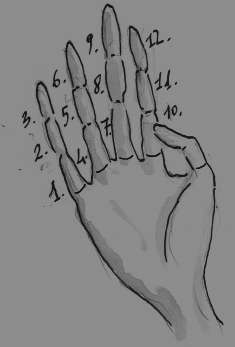
\includegraphics[width=0.3\textwidth]{figs/fingers.png}
\caption{手写数字识别}
\label{手写数字识别}
\end{figure}

以手写字母识别(如图\ref{手写数字识别}）为例，手写字母在形态上具有高度的变化性和不确定性。不同人书写的“A”可能形态差异很大，甚至同一个人也会因速度、情绪等不同而写出不同的“A”。
如果让Logic Theorist识别手写字母"A"和"B"，它会陷入困境，因为符号主义AI依赖预先设定的规则进行逻辑推理，要求字母形态稳定且符合固定定义。而现实中的手写字母形态多样，难以满足这些硬性规则，因此，符号主义AI在这种不确定、变化多样的环境下表现不佳。

虽然这些早期AI系统在模拟人类逻辑推理能力上取得了成功，能够解决简单的逻辑问题，但在面对复杂多变的现实问题时，它们的表现力和适应性明显不足，难以应对更广泛的智能任务。这一局限性表明，符号主义AI在处理现实中的不确定性问题时仍面临巨大挑战。

\subsection*{自我学习}
与此同时，AI研究者也开始探索机器学习的可能性，机器学习领域获得不少突破。1959年， {\bf 阿瑟·塞缪尔}（Arthur Samuel）研制了一款跳棋程序，能够通过自我对弈提升棋艺。1962年，它击败美国州冠军。这款程序被认为是早期{\bf 机器学习}的范例，展示了机器通过经验不断提高性能的潜力，标志着AI研究从预设规则向基于学习的方向发展。1956年，Selfridge 研制出第一个字符识别程序，开辟了模式识别这一新领域。

\subsection*{1974-1980年代初：第一次“AI 寒冬”}

虽然早期的符号AI研究取得了显著进展，但随着研究的持续推进，符号AI的局限性日益显现。尽管符号AI擅长逻辑推理，且在特定任务上表现出色，但在应对现实世界的复杂性和不确定性问题时，特别在处理非结构化数据方面，表现出了明显的不足。

1965年，机器定理证明领域遇到了瓶颈。例如，计算机推了数十万步也无法证明“两个连续函数之和仍是连续函数”。萨缪尔的跳棋程序停留在了州冠军的水准，难以突破。
更糟糕的问题出现在{\bf 机器翻译}领域，计算机在自然语言理解与翻译中表现得极其差劲。例如，翻译程序将英语句子“The spirit is willing but the flesh is weak.”（心有余而力不足）翻译成俄语，再回译成英语时，得到的句子竟变成了“The wine is good but the meet is spoiled.”（酒是好的，肉变质了）。这种笑话般的错误凸显出符号AI在处理语言模糊性方面的无力。

1970年代的乐观情绪（如通用智能）推动了大量AI项目的启动，然而，随着这些项目未能达最初的预期，尤其是在应对现实世界的复杂性方面暴露出显著局限，加上计算资源需求高，导致了随后1974年开始的第一次“AI寒冬”---投资者和政府机构对AI研究的资金支持大幅削减，研究热情和社会关注下降， 许多AI项目被取消，研究活动在1974年至1980年间大幅缩减，AI研究陷入低谷期。

尽管如此，低谷期的AI领域并非全无进展，反而通过知识工程和专家系统的兴起找到了新的突破口。

\section{1980年-1987年：专家系统与知识工程的兴起} 
从1980年至1987年，AI研究进入了一个新的阶段，以{\bf 专家系统}和{\bf 知识工程}的兴起为代表。
美国计算机科学爱德华•费根鲍姆指出，传统的人工智能过于强调通用求解方法的作用，忽略了具体的领域知识。因此，他提出了基于知识的专家系统。
{\bf 知识工程}是利用人工智能技术来构建专家系统的一种方法。{\bf 专家系统}是基于符号逻辑的AI系统，通过将专家的知识编码为计算规则，帮助机器在特定领域中进行推理和决策，模仿领域专家解决问题的过程。 

\subsection{代表性专家系统}

典型的专家系统包括医学诊断系统{\bf MYCIN} 和化学分析系统{\bf DENDRAL}，它们分别在医疗和化学领域取得了显著成效。
通过嵌入领域专家的知识，专家系统在复杂任务中展现出较高的决策能力，推动了知识工程成为AI研究的重要分支。

\begin{itemize}
\item {\bf DENDRAL}：开发始于 1965 年，由斯坦福大学的爱德华·费根鲍姆（Edward Feigenbaum）和约书亚·莱德伯格（Joshua Lederberg）带领的团队创建。DENDRAL则是一种用于化学分析的系统，能够根据分子结构推断化学物质。它被认为是第一个成功的专家系统，标志着知识工程的开端。

\item {\bf MYCIN}：开发始于 1972 年，由斯坦福大学的布鲁斯·布坎南（Bruce Buchanan）和爱德华·肖特利夫（Edward Shortliffe）领导的团队创建。MYCIN是一个医学专家系统，专注于诊断血液感染并推荐抗生素。它通过一系列规则模拟专家在诊断细菌感染时的决策过程， 其规则系统和推理机制为后续专家系统的发展影响深远。 
\end{itemize}

虽然 DENDRAL 和 MYCIN 的开发始于 1960 年代末至 1970 年初，但它们在 1970 年代后期到 1980 年代中期得到实际应用和广泛推广，成为知识工程的核心。
这些专家系统的成功验证了知识工程的可行性。各种专家系统陆续涌现，尤其在疗、化学分析、工程设计和商业决策等特定任务中，标志着AI技术的一个实用转变。
研究者们从这些成功中看到了基于知识的 AI 应用的巨大潜力，开始着重于知识获取、知识表示和推理机制的系统性开发。这一时期成为专家系统和知识工程在实际应用中迅速扩展的高峰期。

\subsection{知识表示与规则推理}
专家系统的成功得益于对{\bf 知识表示}和{\bf 推理机制}的深入研究。{\bf 知识表示}是指如何在计算机中存储和处理专家的领域知识，而{\bf 规则推理}则是通过符号操作来进行逻辑推理的过程。在专家系统中，领域专家的知识被转换为计算机可以处理的规则集，从而模拟专家的判断。这种规则系统让计算机能够在特定领域中像人类专家一样做出高效的决策。

\subsection{ 知识工程的广泛应用}
DENDRAL 和 MYCIN 的成功验证了知识工程的可行性后，推动了更广泛的行业应用。知识工程通过获取和编码人类专家的知识，为 AI 系统提供了专业化的领域知识，并形成了软件产业的一个新分支。知识工程的兴起不仅推动了专家系统的广泛应用，也促成了AI技术在全球范围内的合作和竞争。

受知识工程的激励，日本的第五代计算机计划、英国的阿尔维计划、西欧的尤里卡计划、美国的星计划和中国的863计划陆续推出，
尽管这些计划的目标并不完全针对AI，但AI是其重要组成部分，成为提升国家科技竞争力的一部分。

\subsection{新兴技术：模糊逻辑与贝叶斯网络}
在这一时期，AI领域还从知识工程中衍生出了新的学科分支，如{\bf 模糊逻辑}和{\bf 贝叶斯网络}。模糊逻辑提供了一种处理灰色区域的推理方式，使AI能够在信息不完全的情况下也能做出决策。贝叶斯网络则通过统计方法来处理不确定性，被广泛应用于诊断、预测和决策系统中。这些方法通过处理不确定性和模糊性，有效弥补了传统符号主义AI在处理复杂现实问题上的局限。

\subsection{第二次“AI 寒冬”的反思与转型}
20世纪80年代中期，专家系统和知识工程在医疗诊断、工程设计、化学分析等狭窄领域表现出色，但伴着随大量实践的累积，其局限性也逐渐显现。{\bf 知识获取}成为了最大的瓶颈：专家系统高度依赖领域专家的知识输入和精确的规则，知识获取和维护成本高昂，系统缺乏灵活性和自适应性，难以应对多样和动态的现实需求。此外，硬件技术和计算资源的限制也不足以支撑更大规模的AI系统发展。

随着专家系统的商业化受阻，AI进入了第二次寒冬。
1987年至1993年之间，投资者和政府逐渐减少了对AI的资金支持，许多原本大规模投资的AI项目被迫中止。日本的“第五代计算机计划”因未能在智能计算取得预期成果而停滞，其他国家的大型AI项目也相继缩减，导全球范围内的AI研究热潮急速降温。在这次寒冬期内，AI研究的资金大幅削减，许多研究人员转向其他领域。

第二次的AI寒冬虽然带来了低谷，却促使AI领域反思技术路径，重新审视符号主义AI的局限性。研究者和行业逐渐认识到，仅凭符号规则和知识编码不足以实现真正的智能。

知识工程和专家系统的应用展现了AI技术在特定领域的应用潜力，推动了AI从学术研究向实用化的转变。尽管专家系统存在明显局限，但这些实践经验和技术积累为之后的机器学习、神经网络等数据驱动方向的复兴提供了宝贵启示，推动AI研究进入了新的发展阶段。

寒冬的沉寂期反而带来了新的视角，促使研究者在方法和技术上寻求突破和创新。这些反思和积累成为推动AI转型的重要动力，为现代AI的崛起，尤其是后续深度学习的发展，奠定了坚实的基础。

\section{人工智能的分化}
 1987年以后，人工智能分化为六大学科：
\begin{itemize}
\item 计算机视觉(模式识别，图像处理等)
\item  自然语言理解与交流(语音识别、合成、对话等) 
 \item 认知与推理(各种物理和社会常识等)
\item 机器学习(各种统计建模、分析工具和计算方法)
 \item 机器人学(机械、控制、设计、运动规划、任务规划等)
 \item 博弈与伦理(多代理人agents的交互、对抗与合作、机器人与社会融合等)
\end{itemize}

\begin{figure}[htbp]
\centering
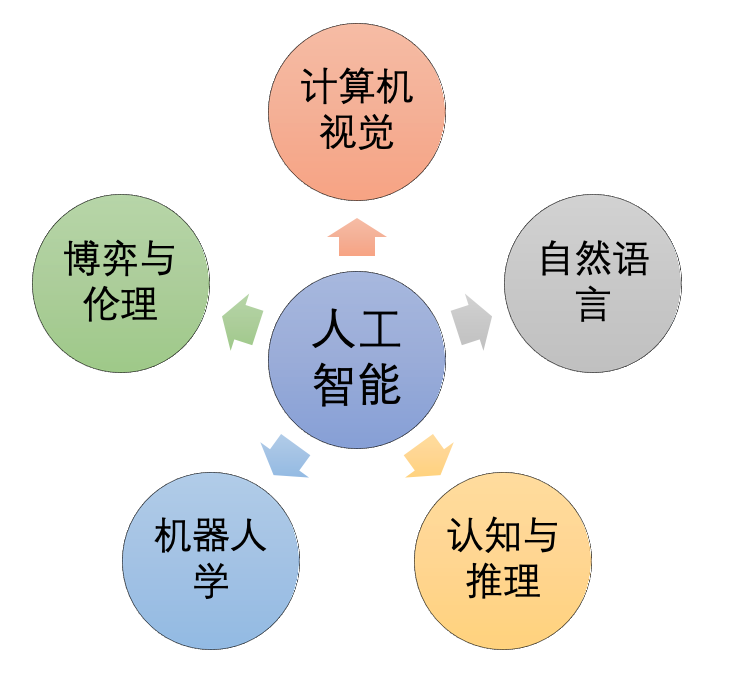
\includegraphics[width=0.3\textwidth]{figs/partition.png}
\caption{“1987年后人工智能的分化”}
%\label{}
\end{figure}

\begin{figure}[htbp]
\centering
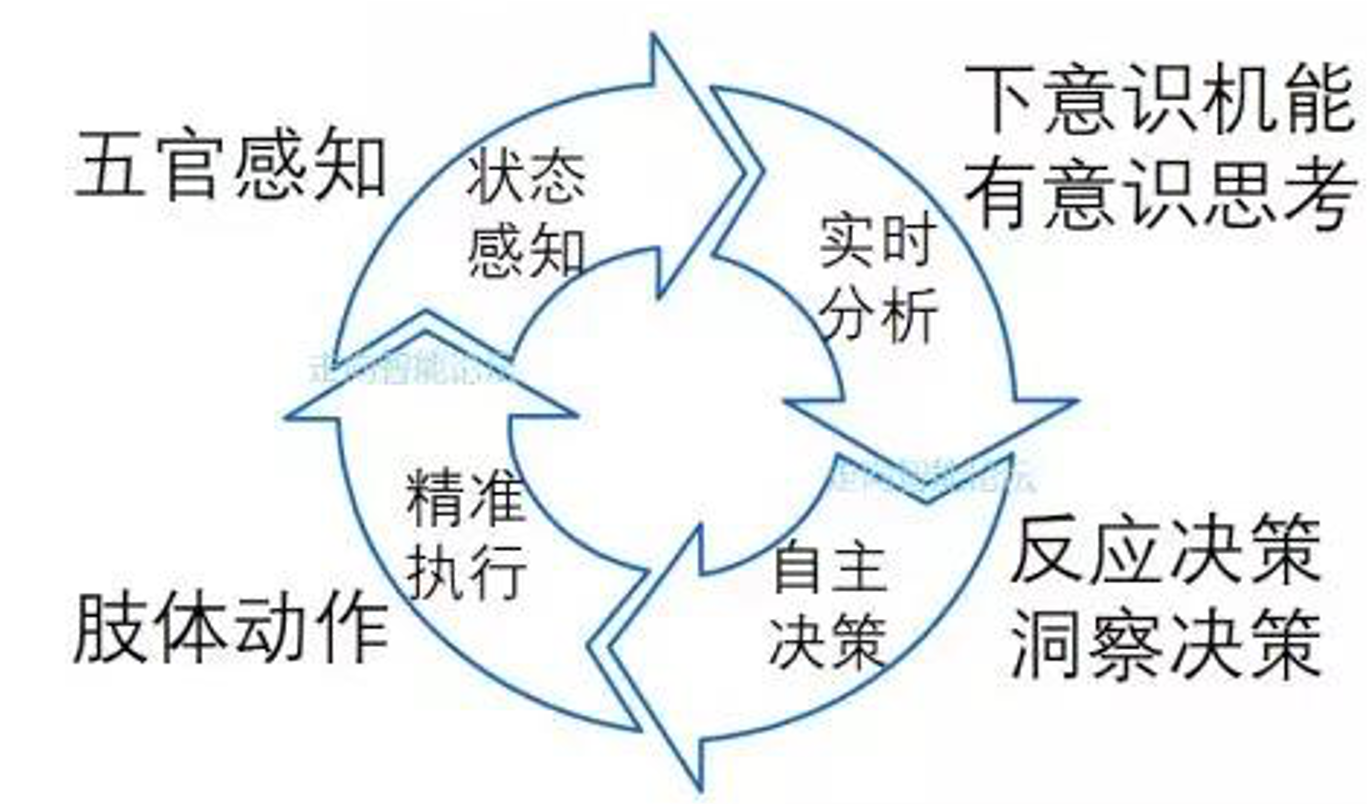
\includegraphics[width=0.3\textwidth]{figs/bio_intelligence.png}
\caption{“1987年后人工智能的分化”}
%\label{}
\end{figure}


\begin{figure}[htbp]
\centering
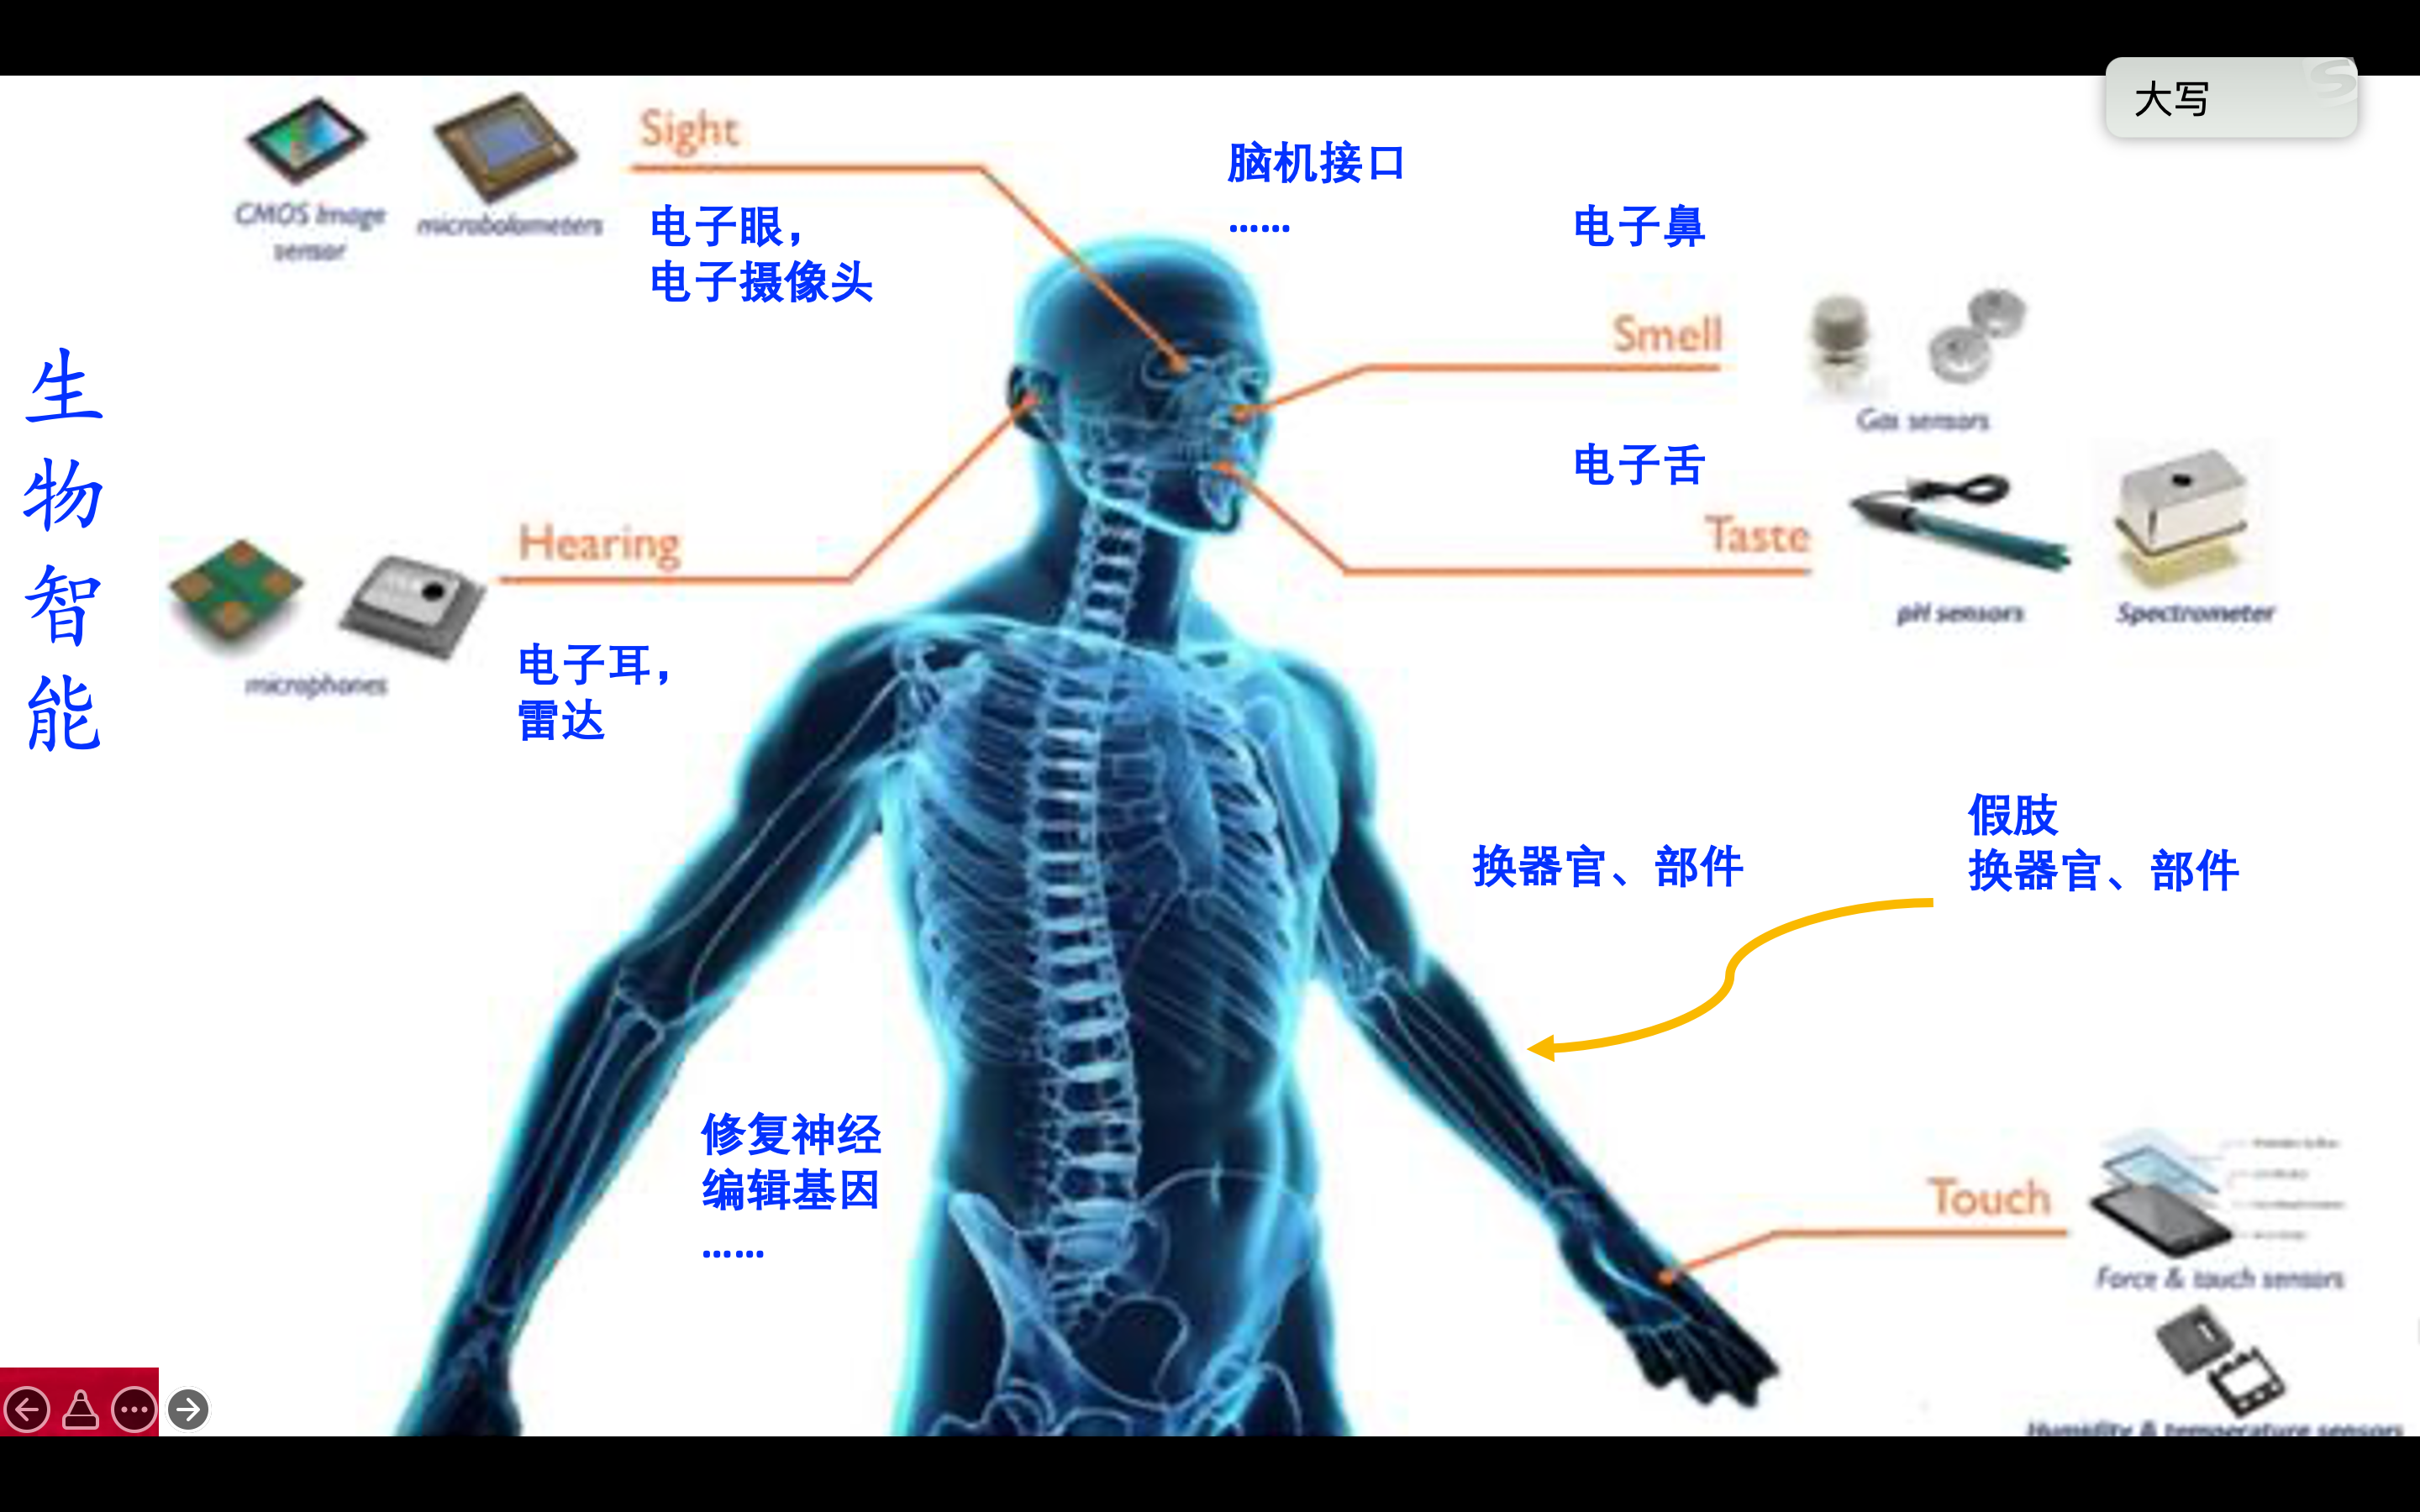
\includegraphics[width=0.3\textwidth]{figs/human_intelligence.png}
\caption{“1987年后人工智能的分化”}
%\label{}
\end{figure}

可以看出来，人工智能在全面模拟人的智能，不仅是大脑智能，还包括眼睛智能，耳朵智能，手智能，口智能。

\section{1990-2010年代：联结主义和机器学习的兴起}

20世纪80年代，{\bf 机器学习}由原本的边缘分支成为关注的焦点。
研究者发现，如果采用完全不同的世界观，即让知识通过自下而上的方式涌现，而不是让专家们自上而下地设计出来，机器学习的问题其实可以得到很好解决。

自下而上的涌现智能的方案很早就提出过，但没有引起注意：
 	一批人：可通过模拟大脑结构（神经网络）来实现(联结学派)
 	另一批人：可从那些简单生物体与环境互动的模式中寻找答案(行为学派)
 20世纪80-90年代，传统的人工智能符号学派、联结学派、行为学派三足鼎立。

早期的学习算法开始在符号AI的基础上发展，成为AI从符号主义向数据驱动方法转型的基础。

尽管1987-1993年期间的AI“寒冬”导致研究资金减少，学术界对神经网络等方向的探索仍在继续。特别是在1990年代后期，联结主义和机器学习的复兴为AI注入了新的活力。研究者们开始着力于数据驱动的学习算法，这些研究逐步成为现代AI，尤其是深度学习的起点。

进入90年代后，AI研究逐渐从符号主义(基于符号的AI)转向数据驱动的机器学习({\bf 基于数据的AI})。在计算机能力提升和数据量爆发增长的推动下，机器学习逐渐成为AI研究的主流。通过统计学习和数据驱动的模式识别，A系统能够大数据进行训练，显著提升识别和决策的准确性。

在这一阶段，{\bf 神经网络}的复兴尤为关键。虽然早期的神经网络（如感知机）在1960年代就已提出，但因计算能力受限，没有达到理想效果。1990年代后，神经网络在计算能力提升的推动下重新焕发生机，显示出巨大潜力。{\bf 1997年，IBM的“深蓝”战胜国际象棋冠军卡斯帕罗夫}，标志着AI在某些特定任务上的重大突破，成为该领域的重要里程碑。

到了2010年代，{\bf 深度学习}技术的突破推动了AI的飞速发展。基于{\bf 卷积神经网络}（CNN）和{\bf 递归神经网络}（RNN）等深度学习模型的广泛应用，AI在图像识别、语音识别、自然语言处理等多个领域取得了显著进展。2012年，{\bf AlexNet}在ImageNet竞赛获胜，奠定了深度学习在图像识别领域的领先地位。2016年，谷歌的{\bf AlphaGo}战胜围棋世界冠军李世石，进一步展示了深度学习和强化学习在复杂问题处理上的强大能力，为AI新时代拉开了序幕。

\subsection{2020年代：大语言模型（LLM）与生成式人工智能（AIGC）的崛起}
进入2020年代，人工智能在语言处理和内容生成领域迎来了崭新的突破。{\bf 大语言模型（LLM）}和{\bf AI生成内容（AIGC）}技术的兴起，标志着AI在自然语言理解、图像生成等跨模态任务上的重大进展。这一阶段的AI系统不仅限于执行特定任务，还展示出强大的语言生成和创意能力，推动了AI在内容生成、对话系统、设计创作等多元领域的应用。

{\bf 大语言模型（LLM）}通过海量文本数据的训练和数十亿参数的深度优化，使得AI具备了对自然语言的复杂理解和生成能力。GPT系列、BERT等模型的出现，让AI能够生成具有上下文连贯性和逻辑性的文本内容，实现更自然、更智能的人机互动。这些模型不仅能处理简单的文本任务，还能在医学、法律、科技等领域为人类提供辅助性建议。LLM的创新，尤其在教育、客服和专业问答等领域的广泛应用，使得AI能够更深入地理解和模拟人类语言的多样性和细腻性，逐步拓宽了人工智能的应用范围。

与此同时，{\bf AI生成内容（AIGC）}技术使AI从信息处理者发展为创意生成者。AIGC让AI不仅可以理解和操作文本，还能够在图像、视频、音乐等领域生成内容，为人类的创意需求提供助力。例如，基于扩散模型和生成对抗网络（GANs）的图像生成器能够创作出栩栩如生的图像，甚至具备了艺术创作的初步能力。AIGC技术使AI在广告、娱乐、设计和教育等多个领域得到了广泛应用，不仅缩短了内容创作的时间，还为人类的创作过程带来了新鲜的灵感和可能性。

LLM和AIGC的兴起不仅丰富了AI的应用场景，更重要的是，它让AI在情感识别、语言生成和创意表达方面具备了更强的适应性，使得AI从单纯的“工具”逐渐演变为可以合作、创新的“伙伴”。AI能够生成具有人性化特质的内容，从而在客服、医疗和心理咨询等对人类情感需求更高的领域中提供更加贴近人类需求的服务。

2020年代的LLM和AIGC的进展，标志着AI从知识服务者走向创意合作者的转变。这一阶段的AI不仅展示了生成文本、图像等复杂内容的能力，也在理解人类表达和模拟创意思维上迈出了一大步。LLM和AIGC带来了前所未有的机遇，将继续推动AI技术在更多领域的应用与普及，引领人类进入一个充满创新和智慧的新时代。

\section{人工智能主要学派}

人工智能从诞生至今，经历了一次又一次的繁荣与低谷，其发展历程大体上可以分为“推理期”，“知识期”和“学习期”。\cite{周志华2016} 

在人工智能的研究中，不同学派以各自的方法和理论基础探索智能的本质。这些学派的差异体现在如何定义智能、模拟智能的方法以及应用的领域中。三大主要学派包括{\bf 符号主义学派}、{\bf 联结主义学派}和{\bf 行为主义学派}，它们分别代表了对智能问题的三种主要思维方式。

\subsection{符号主义学派 (Symbolicism)}

\subsubsection*{符号主义学派：知识驱动的推理与表现}

{\bf 符号主义学派}，又称{\bf 逻辑主义}或{\bf 符号处理学派}，是AI发展的早期重要分支之一。符号主义学派的理论基础源于20世纪中期的认知科学和数理逻辑。
符号主义学派主张，人类的知识和认知可以通过符号加以形式化，且问题解决可以通过符号操作（如逻辑推理）完成。因此，符号主义学派主要专注于建立规则和逻辑系统，尝试通过符号和规则来模拟人类的高级思维过程，包括推理、规划和知识表示。

符号主义学派基于对问题的“高阶”解释，核心思想是智能行为能够通过逻辑规则和知识库来模拟，依赖于启发式搜索和基于规则的推理系统，试图用知识与经验的积累来填补信息空白。这种“If-then”式的推理方式使符号主义在规则明确的任务中表现出色，被广泛应用于医疗诊断、金融分析等领域的专家系统。

\subsubsection*{符号主义学派的成果与应用}
符号主义学派的代表性成果包括早期的专家系统（如MYCIN和DENDRAL）、逻辑定理证明系统（如Logic Theorist）、推理系统和象征性规划系统。

\begin{itemize}
\item {\bf 人机对弈：“深蓝”战胜卡斯帕罗夫}  
  1997年5月11日，IBM的超级计算机“深蓝”在国际象棋比赛中战胜了国际象棋大师卡斯帕罗夫，标志着符号主义AI的一次里程碑事件。深蓝经过四位国际象棋特级大师的训练，储存了100年来几乎所有国际特级大师的开局和残局下法，利用启发式搜索可在1秒钟内计算两亿步棋。这种超强搜索能力，使得“深蓝”通过规则匹配和快速推理“险胜”人类选手，显示了符号主义在明确规则系统中的强大计算能力。
  
\item {\bf 知识问答：Watson战胜人类选手}  
 2011年2月14-16日，在《危险》问答比赛中，IBM的超级计算机Watson战胜人类选手。Watson是个自然语言处理高手。它能够快速理解主持人的提问，并调用广泛的知识库回答问题。它的知识涵盖时事、历史、文学、科学、艺术、流行文化、体育、地理、文字游戏等多个领域，甚至理解语言的隐含意思，比如字谜和双关语，甚至还装满诸如莎士比亚戏剧的独白。Watson 充分体现了符号主义AI在自然语言理解和知识问答中的突破性进展。  

\item {\bf 医疗应用：Watson Health}  
  IBM Watson还被应用于医疗领域，基于大量医学数据和患者数据，为药物研发和个性化健康管理提供支持。例如，在癌症免疫治疗方面，Watson从数百万篇医学论文的2500万篇摘要、400万条病人数据以及1861年以来的药物专利中提取信息，为个性化治疗提供方案。此外，在糖尿病管理上，Watson能够对来自1万名匿名患者的电子健康记录、医保数据和其他公共数据进行实时分析和预测，提前3-4小时预测血糖波动，预测准确率达75-86\%，帮助患者有效管理健康。
\end{itemize}

\subsubsection*{符号主义AI的优势与局限}

符号主义具有以下优势：

\begin{enumerate}
\item   {\bf 可解释性}：符号主义的推理过程与人类的思维方式基本一致，因而具有很强的可解释性，使人们能够理解和追踪系统的推理过程。
\item   {\bf 鲁棒性强}：符号规则系统在处理结构化、规则明确的问题时表现出色，具有较高的稳定性，尤其适用于特定领域内的任务。
\item {\bf 逻辑推理能力}：符号主义系统能够执行复杂的逻辑推理，适用于处理涉及高级认知的任务，如规划和知识表示等。
\end{enumerate}

 20世纪80年代后，符号主义学派的发展逐渐减缓，主要原因在于其依赖的“演绎逻辑和语义描述”以及或“形式化方法”不可能为所有的对象建立模型。
 符号主义系统需要对问题抽象出一个精确数学意义上的解析式数学模型，通过构建理想的数学模型和逻辑规则来模拟智能行为。一旦模型建立，计算任务与能力就被唯一地确定。
 确定的算法无法表示现实世界问题所固有的测不准性和不完备性：世界是动态的、复杂的，无法用一个模型来表达。
此外，图灵意义下的可计算问题都是可递归的，但可递归并不是解决问题的唯一途径。虽然符号处理可以应对某些递归性问题，但对于智能的全面理解和表现，符号主义学派的框架显然不够完整。

符号主义学派的主要局限性可归纳如下：
\begin{enumerate}
\item    {\bf 知识依赖性}：符号主义系统依赖于大量准确、结构化的知识和规则，但人类知识难以全面准确地形式化，这种依赖性限制了系统在现实问题中的表现。
\item   {\bf 缺乏灵活性}：符号主义系统只能应对预先定义的问题，难以适应动态、复杂和不确定的环境。这种限制使其在处理非结构化问题时表现不佳。
\item   {\bf 条件与分枝问题}：在复杂的动态系统中，符号主义面临两大瓶颈：{\bf 条件问题(Qualification Problem)}，即难以穷尽智能行为的所有先决条件；{\bf 分枝问题(Ramification Problem)}，即无法枚举智能行为的所有隐含结果。符号主义系统因此难以应对复杂环境中的不确定性和隐含影响。
\item   {\bf 应用领域狭窄}：尽管符号主义模型在逻辑推理和规则明确的任务中表现出色，但在感知、语言理解等模糊和动态性较强的任务中，由于对人工定义的规则和知识库的依赖，其适应性较差。
%符号主义系统依赖于大量准确、结构化的知识和规则，但人类知识往往难以全面准确地形式化，导致系统在处理现实问题时缺乏灵活性。符号主义系统只能应对预先定义的问题，难以处理动态和不确定的现实环境。此外，在复杂的动态系统中，不可能穷尽所有先决条件（条件问题）或智能行为的所有潜在结果（分枝问题），因此符号主义模型在应对复杂环境和不确定性时表现不佳。尽管符号主义模型在逻辑推理等规则明确的任务上擅长应用，但在感知、语言理解等模糊和动态性较强的任务中，由于其对规则和知识库的人工依赖，适应性较差。
  \end{enumerate}
 
 符号主义学派在AI发展的早期取得了显著成就，为人类理解和模拟智能行为提供了框架和方法。然而，随着应用需求的增加和技术环境的变化，符号主义的局限性逐渐显现，学界认识到，为应对复杂的动态环境，还需结合其他学派的思维方式。符号主义的贡献在于奠定了知识驱动的AI基础，展示了通过逻辑推理模拟人类智能的可能性，为之后联结主义与行为主义的发展开辟了道路。

\subsection{联结学派/连接学派(Connectionism)：从神经网络到深度学习}
 20世纪80年代之后，随着计算能力的提升和神经科学的深入研究，人工智能的重心逐渐转向{\bf 联结主义学派}，也称{\bf 人工神经网络学派}。联结主义学派认为智能的产生并非依赖于符号和逻辑规则，而是源于大脑中成千上万个神经元的联结和计算。正如其支持者所言，“高级的智能行为是从大量神经网络的连接中自发出现的”。
  
联结主义学派主张通过模仿大脑神经元网络的工作原理来实现智能。大脑由一万亿个神经元细胞通过错综复杂的相互连接形成了复杂的认知和决策能力。
特别关注如何通过数据训练来自动调整网络参数，使系统能够在数据中自发学习和优化。
其核心思路是模仿神经元的工作方式，构建多层网络结构，调整神经元之间的连接权重，使得系统逐渐具备特定的识别和判断能力。
例如，神经网络的训练过程就是通过不断调整权重，逐步优化输出结果的过程。不同于符号主义学派的知识驱动，联结主义的这一训练机制强调{\bf 数据驱动的学习}，即依靠大量的数据输入，使系统在学习中自动调整网络参数，以形成稳定的模式识别和分类能力。

联结主义学派的重要进展包括从早期的{\bf 感知机模型}到更复杂的{\bf 卷积神经网络}（CNN）、{\bf 递归神经网络}（RNN）等模型，最终发展到现代{\bf 深度学习}模型。这些模型推动了AI在图像识别、自然语言处理、生成式AI等领域的广泛应用，成为现代AI的重要工具。这一学派的成就在近年来引发了广泛关注和思考。

尽管联结主义学派推动了人工智能的飞跃式进展，但其局限性也不容忽视。首先，联结主义模型对大量数据的依赖较高，若数据不足或质量不佳，模型的表现可能会大幅下降。其次，随着神经网络层次增加，其计算复杂度也随之提高，导致训练和运行成本显著增加。其次，神经网络通常被视为“黑箱”，即难以解释其内部决策依据。这一“黑箱”问题主要源于以下几点：
\begin{itemize}
\item {\bf 多层非线性结构：}神经网络的层层变换过程使其难以还原具体决策路径，庞大的参数量也导致分析“哪些特征在决策中起了关键作用”变得困难。
\item {\bf 局部特征依赖性：}模型往往基于局部特征组合来进行决策，而缺乏对整体决策过程的全局视角。例如，在图像分类中，模型可能依赖某些局部图案作出决策，使得预测依据难以解读。
\item {\bf 数据驱动缺乏推理链：}联结主义模型倾向于基于统计特征进行预测，缺乏类似符号主义系统的逻辑推理链，不便于展示推理过程。
\end{itemize}

%针对神经网络的“黑箱”问题，研究者们尝试通过可视化、解释性模型（如LIME和SHAP）、知识蒸馏等技术来改善神经网络的可解释性，使其在医疗、金融等领域获得更高的应用价值。
尽管存在可解释性方面的挑战，联结主义的理论和技术构建了现代神经网络的基石，极大地推动了现代AI的发展。在下一章中，我们将进一步探讨联结主义的核心思想、模型结构及其应用实践。

\subsection{行为主义学派(Actionism)}

{\bf 行为主义学派}源于20世纪中叶，其理论基础来自行为主义心理学和生物学对动物行为的研究，认为智能体可以通过与环境的交互获得经验，从而逐步学习最优的行为策略。行为主义学派主张智能的形成基于行动与环境反馈的相互作用，智能体在反复试错中调整自身策略，优化行为序列，以实现既定目标。

行为主义学派的早期探索主要集中于模仿昆虫等低等生物的行为模式。简单生物无需复杂的大脑结构，也不会按照传统的方式进行复杂的知识表示和推理来执行智能行为，仅通过直接的环境交互就能实现适应性行为。例如，昆虫能够灵活移动、快速反应、躲避捕食者的攻击；小小的蚂蚁所组成的庞大蚁群展现出高度写作的群体智能。这些生物体的行为为行为主义学派提供了灵感。 随着计算能力的提升，行为主义方法逐渐被应用于机器人控制、游戏策略等领域，特别适合在高不确定性和动态环境中构建智能体行为。

行为主义学派的一个典型实现是{\bf 强化学习}（Reinforcement Learning, RL）算法，尤其是Q学习和深度强化学习（DRL）。这些方法通过奖励机制引导智能体在环境中逐步优化策略。例如，AlphaGo挑战围棋世界冠军的成功便是强化学习和深度学习结合的成果。AlphaGo在与环境的持续交互中，逐步学习复杂博弈中的最佳策略，展示了人工智能在自我优化和复杂决策方面的潜力。

MIT机器人专家Rodney Brooks设计的模仿昆虫的机器人正是这一学派的经典案例。通过四肢和关节的协调，这些机器人能够在复杂地形中灵活爬行，巧妙避开障碍物，无需复杂的大脑控制。类似地，波士顿动力公司（Boston Dynamics）开发的四足机器人在不同地形和环境中表现出高度的适应性和鲁棒性。
这些机器人的行为不依赖于复杂的认知模型或高级符号推理，而主要依靠局部传感器数据、反馈控制和运动算法来实现稳定的运动与环境适应，在一定程度上可以被称为“无脑机器人设计”。这种设计理念类似于昆虫等简单生物的直接感知-行动环的反应式行为，展示了行为主义学派在机器人开发和运动控制中的实际价值。

尽管行为主义学派取得了诸多进展，仍面临明显的局限性：

\begin{enumerate}
\item {\bf 高维度和复杂环境下的学习效率低：}行为主义学派在高维、复杂环境中往往需要大量交互才能收敛到合理策略，试错成本较高。
\item {\bf 奖励依赖：}行为主义模型依赖奖励反馈引导学习，当目标明确时效果良好，但在奖励稀疏或模糊的情况下，学习效果可能较差。
\item {\bf 难以实现高阶智能的自然涌现：}尽管行为学派在模仿昆虫和群体智能方面取得了一定成果，但对于实现更高层次智能行为的涌现机制，行为学派难以给出明确解释和实现路径，%回答“在什么条件下会发生智能涌现”或“如何设计底层规则来产生预期的智能行为”，
因此在复杂任务的应用中受到限制。
\end{enumerate}

尽管行为学派在模拟高级智能方面仍有不足，其在机器人技术、自动驾驶等实际应用中展示了极强的适应性和应用潜力。

%行为主义学派中的一支，**进化计算**，通过模拟自然选择来优化智能体行为，采用遗传算法、进化策略等方法，不需要将学习区分为训练和执行两个阶段，而是在执行过程中持续优化策略。这种“学习中执行”的方式为行为主义学派在应对不确定性环境中的适应性提供了新的思路。
%与神经网络不同，遗传算法不需要把学习区分成训练和执行两个阶段，完全可以指导机器在执行中学习learning by doing，比神经网络更具方便表达性和简单性。
%进化计算大家庭：演化策略、演化编程和遗传编程
%\begin{figure}[htbp]
%\centering
%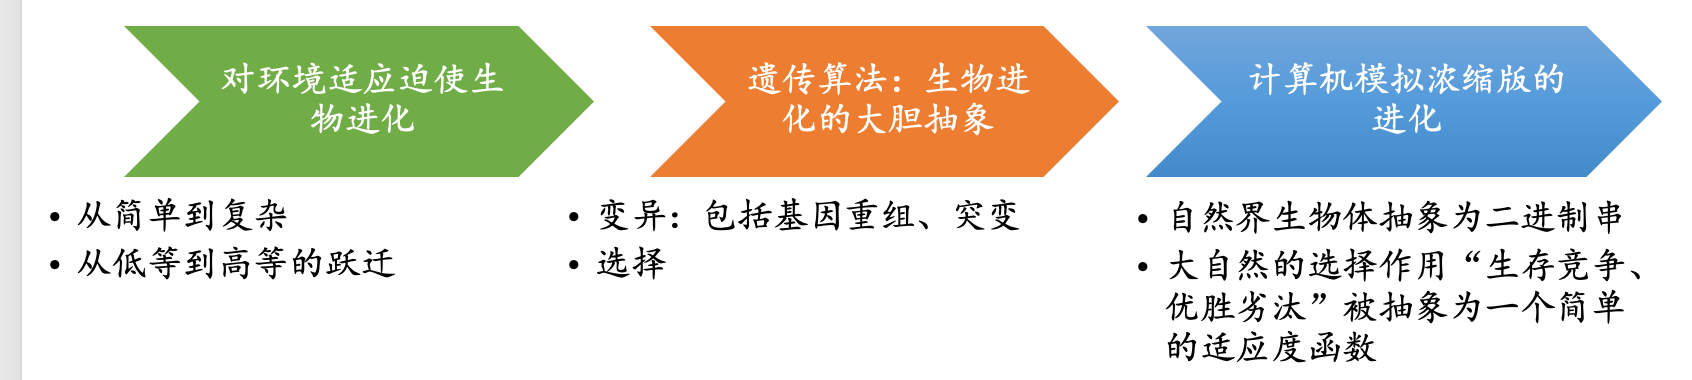
\includegraphics[width=0.6\textwidth]{figs/进化计算.png}
%\caption{进化计算}
%%\label{}
%\end{figure}

\subsection{三大学派的比较}

\subsection{三大学派对比总结}

人工智能的发展经历了显著的转型：从依赖人工规则的符号主义学派，到借助经验和反馈的联结主义与行为主义学派，AI的核心方法从“推理期”和“知识期”逐渐过渡到“学习期”。这种变化反映了AI在应对复杂问题时，从自上而下的规则构建转向自下而上的经验学习。符号主义学派强调人工设计规则和知识库来解决问题，而联结主义学派和行为主义学派则更关注如何通过数据驱动的方式从经验中学习知识。

人工智能发展过程中，{\bf 符号主义学派}、{\bf 联结主义学派}和{\bf 行为主义学派}分别从不同角度探索智能的本质。每一学派都有其独特的理论基础、代表方法和应用领域，也各有特色。
符号学派主要关注智能的逻辑和推理过程，模拟智能软件的工作方式；联结学派则通过模仿大脑神经元结构，试图在“硬件”层面上还原智能；而行为学派则基于简单生物体与环境互动的模式，从动态环境中找寻适应性智能。

\begin{enumerate}
\item {\bf 符号主义学派(传统人工智能)}：以逻辑和符号操作为基础，符号主义学派侧重于通过规则和知识库模拟人类的逻辑推理能力。其典型方法包括基于规则的专家系统，主要应用于知识明确、规则清晰的领域，如医疗诊断和金融分析。
 符号主义的优势在于其强大的可解释性，推理过程清晰可见，便于理解。
 然而，符号主义在处理复杂、不确定的环境时表现有限，因为它依赖于结构化的知识库和固定规则，难以应对环境的动态变化。
 符号主义的知识设计是{\bf 自上而下}的，主要通过逻辑设计和专家知识进行知识建模，但人类的知识和经验往往难以精确描述，并且复杂的推理过程增加了计算难度。

\item {\bf 联结主义学派}：借鉴神经科学，联结主义学派通过构建人工神经网络来模拟大脑的学习和感知机制。其代表模型包括卷积神经网络（CNN）、递归神经网络（RNN）等，强调通过数据驱动的学习，在大规模数据中自动调整参数，广泛应用于图像识别、语音识别和自然语言处理等领域。联结主义学派的优点在于其强大的数据处理能力，可以自适应复杂数据环境；联结主义的知识形成是{\bf 自下而上}的，通过模拟神经网络结构涌现知识。然而，其“黑箱”性质导致可解释性不足，且训练过程依赖大量数据和计算资源。

\item {\bf 行为主义学派}：基于行为主义心理学和生物学对动物行为的研究，行为主义学派强调通过智能体与环境的交互来优化行为策略，其典型实现是强化学习。行为主义方法更适合动态和不确定环境中的智能体训练，例如自动驾驶、机器人控制和游戏对抗。行为主义的特点是其试错式学习机制，使得智能体在持续反馈中逐步优化策略。然而，其高维度环境中的学习效率较低，且高度依赖明确的奖励信号，难以实现对高阶智能的自然涌现。
\end{enumerate}

\noindent {\bf 学派间的比较}：
\begin{itemize}
    \item{\bf 理论基础：}
   符号主义学派依赖符号和逻辑推理，经由专家自上而下基于逻辑来构建知识系统；联结主义学派模仿神经网络的结构，自下而上实现知识的涌现；行为主义学派则从智能体的行动和环境反馈中寻找最优策略，构建出适应性的智能。三者代表了不同的智能观：符号主义偏向于逻辑和推理，联结主义倾向于模式识别和学习，行为主义重视试错与适应。
 
  \item {\bf 适用领域：}符号主义适用于规则明确、知识体系完善的场景；联结主义适合海量数据驱动的模式识别任务；行为主义则在动态、非结构化的环境中表现突出，如自动驾驶和机器人控制。

\item **优劣势**：符号主义具有良好的可解释性，但灵活性有限；联结主义具备强大的感知与模式识别能力，但对数据依赖性高，且可解释性不足；行为主义适应性强，但在高维度和奖励稀疏的环境下学习效率较低，难以实现复杂智能的涌现。
\end{itemize}

三大学派的各自特长和局限使得现代人工智能研究趋向于融合不同方法。例如，将符号逻辑引入神经网络以提升可解释性，或将强化学习与深度学习结合以应对复杂策略任务。通过综合符号推理、神经网络和交互学习的优势，现代AI逐渐朝着多模态、多层次的智能系统发展，在更多领域实现了实际应用。

\begin{table}[htbp]
  \centering
  \caption{三大学派的比较}
  \begin{tabular}{|p{0.1\textwidth}|p{0.27\textwidth}|p{0.27\textwidth}|p{0.27\textwidth}|}
    \toprule
     \centering\textbf{学派}  & \centering\textbf{主要观点}  &\centering \textbf{优势 } &\textbf{ 局限性}   \\
    \midrule
  符号主义   &符号和规则模拟人类智能  &擅长结构化问题和逻辑推理   & 难以处理非结构化和动态环境   \\    \midrule 
   联结主义 & 神经网络模拟大脑联结    &  数据驱动，自动学习  & 需要大量数据，解释性不足   
    \\     \midrule
      行为主义  & 交互和反馈强化行为学习   & 适用于策略优化和动态决策    &  需要大量交互，目标不明确时效率低   \\
    \bottomrule
  \end{tabular}
\end{table}

\begin{table}[htbp]
  \centering
  \caption{人工智能主要学派}
  \begin{tabular}{|p{0.3\textwidth}|p{0.3\textwidth}|p{0.3\textwidth}|}
    \toprule
     \centering\textbf{符号主义学派}  & \centering\textbf{联结主义学派}  & \textbf{行为主义学派} \\
    \midrule
   认知即计算 &认知即网络 & 感知-行动  \\
    \begin{itemize}
\item 起源于2300年前，更关注哲学，逻辑学和心理学，将学习视为逆向演绎
\item 使用符号、规则和逻辑来表征知识和进行逻辑推理
\end{itemize}
 & 
  \begin{itemize}
\item 起源于上世纪40年代，专注物理学和神经科学
\item 使用概率矩阵和加权神经元来动态地识别、分类、归纳
\end{itemize}
&\begin{itemize}
\item 起源于上世纪40年代
\item 在遗传学、进化生物学、控制论的基础上，生成变化，为特定目标获取其中最优解
\end{itemize}
    \\
      {\bf 常用算法：}规则和决策树
 &  {\bf 常用算法：}深度学习神经网络、反向传播 &   {\bf 常用算法：}遗传算法、蚁群算法、强化学习  \\
    \bottomrule
  \end{tabular}
\end{table}

三大学派的方法论

\begin{figure}[htbp]
\centering
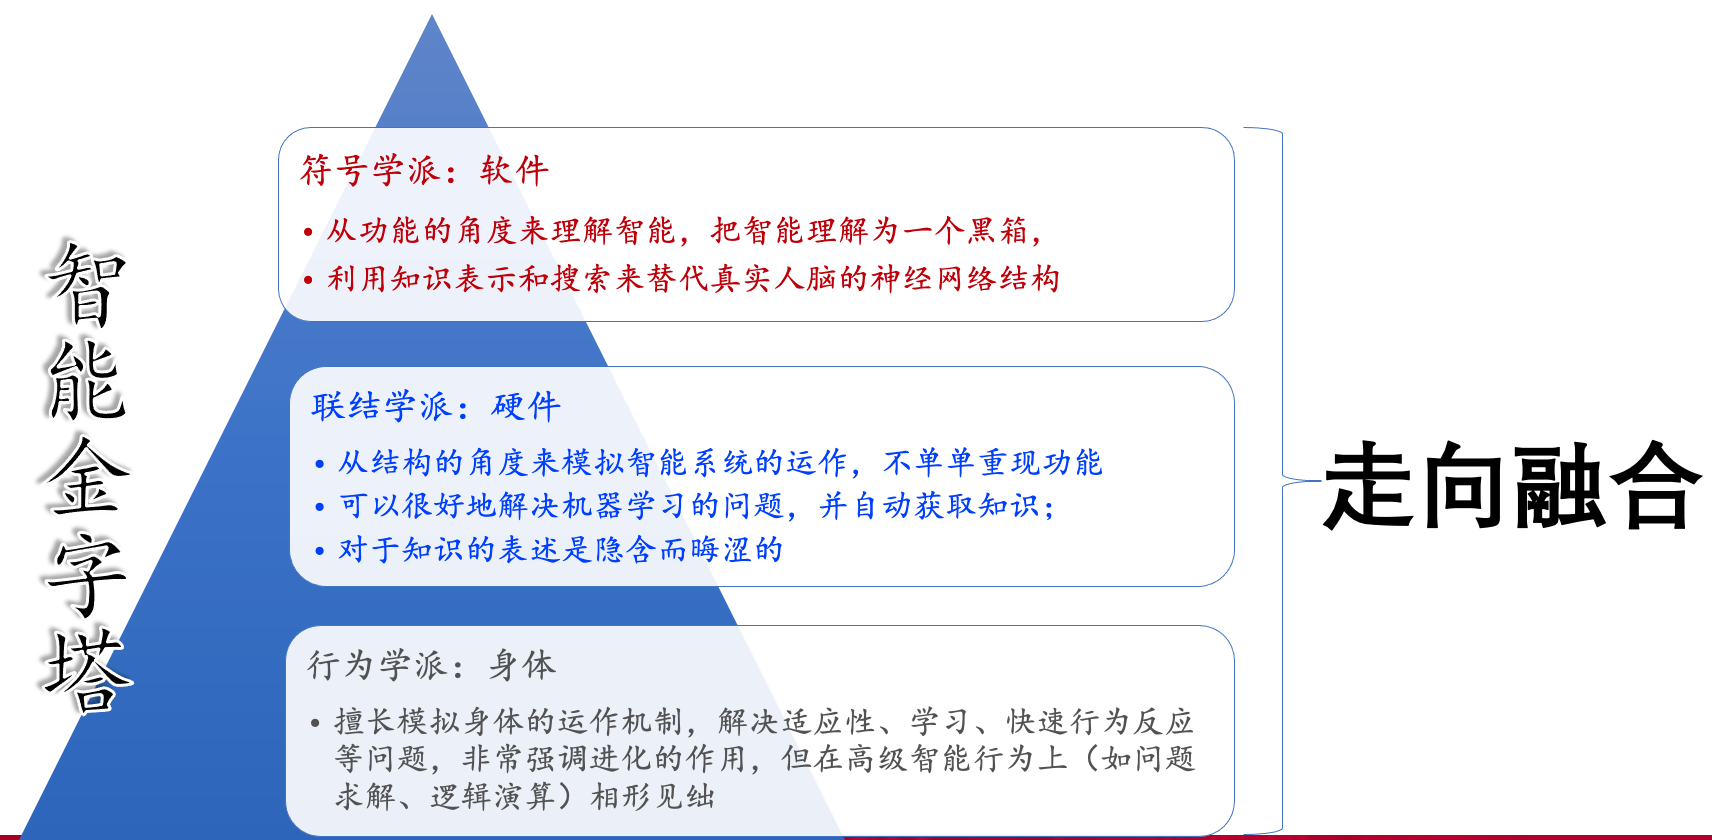
\includegraphics[width=0.9\textwidth]{figs/金字塔.png}
\caption{智能金字塔}
%\label{}
\end{figure}

\section{小结：危机与机遇中的AI发展之旅}

纵观人工智能的成长历程，它既是一场理解智能的探索，也是一场应对挑战的征途。AI的发展如同蜿蜒的河流，经历过激荡的浪潮，也度过了平静的深潭。在数次寒冬的洗礼后，AI不断焕发新的生机，展示出危机中的无限机遇。

每一次技术突破和危机，都塑造了AI的未来方向。

1. {\bf 达特茅斯会议后的开创期（1956年 - 1970年代初）}：1956年的达特茅斯会议首次提出“人工智能”概念，开启了AI的黄金时代。研究者尝试用逻辑推理和符号操作来模仿智能，开发了Logic Theorist和General Problem Solver等符号主义AI的早期成果，虽为初探，却为智能探索奠定了基础。

2. {\bf 第一次AI寒冬（1974年 - 1980年代初）}：
由于符号主义AI无法解决现实问题的模糊性和不确定性，以及高昂的资源消耗，AI研究在此期间陷入低谷，资金支持大幅削减。这场寒冬也促使研究者反思符号主义AI的局限性，重新思考智能的实现路径，为下一阶段的知识工程发展铺平了道路。

3. {\bf 专家系统和知识工程的兴起（1970年代末 - 1980年代中期）}：第一次AI寒冬后，DENDRAL和MYCIN等专家系统展示了AI在医疗、化学分析等领域的实际应用潜力，使AI逐渐从实验室走向商业应用，知识工程兴起。但由于专家系统过度依赖手动编码的知识和固定规则，逐渐暴露出适应性不足的局限。

4. {\bf 第二次AI寒冬（1980年代末 - 1990年代初）}：
专家系统的高昂维护成本和对环境的适应性限制使得全球的AI项目纷纷缩减以至于停滞，AI再次进入低谷。但这场寒冬促使AI领域认识到，仅靠符号规则难以实现真正智能，推动了方法上的转型。

5. {\bf 联结主义和机器学习的崛起（1990年代 - 2010年左右）}：以神经网络和数据驱动方法为基础，联结主义和机器学习的蓬勃发展，标志着AI从符号主义迈向数据驱动的新时代。机器学习逐渐成为主流方法，通过模式识别和大数据训练，使AI具备了在各种任务中自我改进的能力。1997年，IBM的“深蓝”战胜卡斯帕罗夫，这一里程碑事件展现了机器学习在复杂决策中的潜力，也宣告了数据驱动AI的初步胜利。

6. {\bf 深度学习的快速发展（2010年代）}：在计算能力提升和数据量增加的支持下，深度学习技术在图像识别、语音识别、自然语言处理等领域取得突破性进展，使AI再度迎来黄金期。2016年，AlphaGo战胜李世石，标志AI在复杂推理问题上的新高度。寒冬中的积累与反思，转化为深度学习这一数据驱动方法的强大推动力，成就了AI新时代的辉煌。

7. {\bf 大语言模型（LLM）与{\bf AIGC}的崛起（2020年代）}：
近年来，基于数十亿参数和海量数据训练的大规模语言模型（如GPT系列和BERT）与AI生成内容（AIGC）技术迅速崛起。LLM具备深度语言理解和生成能力，能进行逻辑连贯的文本生成，开创了更加自然的智能人机互动。AIGC进一步拓展了AI的创作边界，使AI从信息回答者进化为创意合作伙伴，广泛应用于创意内容生成、广告、教育和娱乐领域。

在危机与机遇交织的AI发展史中，每一次危机都意味着新的机遇。两次寒冬带来低谷，但也促使AI领域在反思中寻找新方向，逐渐摆脱了对符号逻辑的单一依赖，向数据驱动和自适应学习的方向迈进。

知识工程为AI的应用打开了大门，而机器学习和深度学习的崛起则奠定了现代AI的基础。

今天，AI的视野已从实验室扩展到生活的方方面面，从模仿人类思维到自主学习，从专注特定领域到应对复杂决策。AI的历程是一部充满智慧与勇气的进化史，展现了智能的无限潜力。我们期待AI继续向前，为人类揭示智能的更多可能性，并引领我们在未知中发现更广阔的世界。
%---


%伴随着深度学习技术和计算资源的进一步发展，大规模语言模型（如GPT系列和BERT等）和AI生成内容（AIGC）技术迅速崛起。基于数十亿参数和海量数据的训练，这些模型赋予AI深度语言理解和生成能力，从对话系统、文本生成到跨模态的图像生成，广泛应用于创意内容生成、广告、教育和娱乐等行业。
%{\bf 大语言模型（LLM）}能够生成逻辑连贯、具备上下文理解的文本内容，开创了更自然、更智能的人机互动模式。GPT系列模型不仅能够根据用户输入回答问题和生成文章，甚至还能在医学、法律等领域提供专业参考意见，大幅提升AI在自然语言处理方面的能力。
%{\bf AI生成内容（AIGC）}进一步拓展了AI的创作边界，使AI能够创作文本、生成图像和视频，甚至在音乐创作和设计领域展现潜力。这一进展标志着AI从知识回答者进化为创意合作伙伴，将AI的应用从单纯的任务处理扩展到创造性表达，使得AI成为人类思维的强大助力。
%总结
%LLM和AIGC的崛起标志着AI在内容生成和自然语言理解上的跨越式发展，丰富了AI的应用场景，提升了人机互动的智能水平，为AI在未来的普及应用和技术发展奠定了新的基础。


\nocite{*}
\printbibliography[heading=bibintoc, title=\ebibname]


%参考文献：人类计算.冯•安的网站http://www.cs.cmu.edu/~biglou/

\newpage


